\cotefile{148}
\scanpage{12}

\noindent\begin{minipage}[t]{0.43\textwidth}
\centering
U N I V E R S I T E\\
DES SCIENCES ET TECHNIQUES\\
DU LANGUEDOC\\
\textasciicircum\textasciicircum\textasciicircum\textasciicircum\textasciicircum\textasciicircum\textasciicircum\textasciicircum\textasciicircum\textasciicircum\textasciicircum\textasciicircum\textasciicircum
\end{minipage}\hfill
\begin{minipage}[t]{0.49\textwidth}
\raggedleft
\vspace{\baselineskip}
Montpellier, le 14 octobre 1983
\end{minipage}

Service de la Scolarité

Diffusion : Liste A\\
MA/gs \qquad N° 4470

\begin{center}
AVIS DE SOUTENANCE D'UNE THESE DE DOCTEUR-INGENIEUR

`` PHYSIQUE \quad DES MATERIAUX ''

\texttt{====================================================}
\end{center}

\uline{NOM et Prénom du candidat} : GOUDEAU Jacques

\uline{Titre de la thèse} : ``Contraint\unsure{\mbox{e\kern-0.2em{}s}} de trempe thermique dans des pièces à\\
symétrie de révolution''

\uline{Date, heure et lieu de soutenance prévus} : Le 28 octobre 1983, à 11 heures\\
Salle de l'IREM - Université des Sciences et Techniques du Languedoc

\uline{Nom du Directeur de thèse} : M. ZARZYCKI - M. MAISONNEUVE

\uline{Désignation du Laboratoire où la thèse est préparée} : Laboratoire de Sciences\\
des Matériaux, Mécanique des Milieux continus, Chimie structurale - U.S.T.L.

\uline{Analyse de l'ouvrage} : On étudie l'évolution des champs de température et de\\
contraintes, dans une pièce en verre à symétrie de révolution.

Pour cela on résout par éléments finis un problème de\\
thermovisco-élasticité, avec une loi de comportement de type MAXWELL à coefficients\\
variables en fonction de la température.

On compare les résultats obtenus à ceux d'une méthode\\
optique d'analyse des contraintes ainsi qu'à une méthode industrielle de mésure.

\uline{Durée approximative des recherches ayant abouti à la thèse} : 2 ans

\uline{Composition du jury proposé} : \begin{tabular}[t]{ll}
MM. & ZARZYCKI J.\\
& MAISONNEUVE O.\\
& REGNIER J\\
& FRANCOIS\\
& BOURRET D.
\end{tabular}

\begin{flushright}
\begin{minipage}{0.55\textwidth}
\raggedright
P/ le Secrétaire Général,\\
\hspace*{1em}l'Attachée Principale d'Administration\\
\hspace*{1em}Scolaire et Universitaire,

\medskip
% Signature contours; alphabetic reading unresolved.
\hspace*{2.6em}\unsure{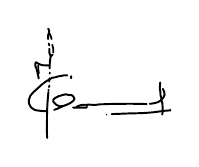
\begin{tikzpicture}[x=0.00083cm,y=-0.00083cm,line cap=round,line join=round]
\draw[line width=0.7pt] (496,250) .. controls (520,262) and (512,292) .. (507,314) .. controls (493,339) and (491,374) .. (496,410);
\draw[line width=0.65pt] (518,327) .. controls (533,350) and (540,381) .. (549,410);
\draw[line width=0.65pt] (503,478) -- (514,509);
\draw[line width=0.65pt] (559,499) .. controls (577,529) and (574,576) .. (573,620);
\draw[line width=0.7pt] (516,560) .. controls (506,603) and (517,650) .. (536,679) .. controls (549,675) and (560,665) .. (566,651);
\draw[line width=0.7pt] (533,684) .. controls (524,749) and (515,802) .. (519,863);
\draw[line width=0.65pt] (520,926) -- (519,945);
\draw[line width=0.7pt] (517,1015) -- (512,1065);
\draw[line width=0.65pt] (516,1128) -- (508,1151);
\draw[line width=0.65pt] (502,1190) -- (501,1212);
\draw[line width=0.7pt] (499,1232) .. controls (488,1344) and (483,1431) .. (479,1521) .. controls (478,1641) and (476,1761) .. (477,1845) .. controls (477,1882) and (479,1910) .. (482,1934);
\draw[line width=0.7pt] (519,815) .. controls (477,815) and (435,818) .. (400,813) .. controls (372,803) and (336,787) .. (309,768) .. controls (298,772) and (295,801) .. (299,830) .. controls (314,851) and (325,886) .. (330,923) .. controls (338,963) and (347,999) .. (351,1018);
\draw[line width=0.6pt] (343,813) .. controls (342,864) and (347,903) .. (353,942);
\draw[line width=0.7pt] (790,971) .. controls (761,959) and (736,974) .. (712,976) .. controls (671,981) and (631,988) .. (599,1002) .. controls (564,1008) and (539,1003) .. (516,1034) .. controls (460,1060) and (409,1100) .. (356,1151) .. controls (301,1200) and (252,1238) .. (220,1287) .. controls (198,1320) and (195,1366) .. (200,1405) .. controls (207,1453) and (249,1485) .. (290,1504) .. controls (344,1518) and (410,1519) .. (479,1524);
\draw[line width=0.7pt] (849,983) -- (851,1015);
\draw[line width=0.7pt] (588,1502) .. controls (647,1485) and (712,1445) .. (783,1422) .. controls (835,1402) and (884,1373) .. (902,1335) .. controls (897,1313) and (882,1288) .. (863,1277) .. controls (840,1267) and (822,1279) .. (802,1271) .. controls (781,1257) and (760,1262) .. (731,1270) .. controls (684,1281) and (633,1297) .. (602,1320) .. controls (577,1333) and (565,1353) .. (576,1380) .. controls (601,1415) and (638,1442) .. (675,1447) .. controls (711,1453) and (751,1439) .. (788,1421);
\draw[line width=0.7pt] (881,1467) -- (1090,1467) -- (1092,1424);
\draw[line width=0.7pt] (934,1453) .. controls (974,1430) and (1014,1425) .. (1072,1423) .. controls (1121,1420) and (1169,1424) .. (1226,1427) .. controls (1281,1413) and (1342,1417) .. (1408,1413) .. controls (1515,1408) and (1628,1410) .. (1742,1408) .. controls (1840,1409) and (1924,1408) .. (2014,1413);
\draw[line width=0.7pt] (2063,1409) .. controls (2101,1400) and (2141,1406) .. (2188,1384) .. controls (2215,1370) and (2230,1360) .. (2241,1345) .. controls (2260,1330) and (2282,1306) .. (2291,1272) .. controls (2293,1239) and (2280,1210) .. (2265,1179);
\draw[line width=0.7pt] (2224,1080) .. controls (2231,1107) and (2209,1131) .. (2216,1167) .. controls (2229,1204) and (2225,1254) .. (2229,1281) .. controls (2233,1307) and (2249,1320) .. (2241,1345) .. controls (2257,1381) and (2262,1423) .. (2261,1470) .. controls (2265,1511) and (2261,1550) .. (2254,1574);
\fill (1395,1576) ellipse [x radius=11,y radius=13];
\draw[line width=0.7pt] (1476,1567) .. controls (1592,1565) and (1693,1557) .. (1807,1556) .. controls (1911,1554) and (2017,1550) .. (2121,1539) .. controls (2209,1530) and (2283,1512) .. (2377,1511) -- (2375,1499);
\end{tikzpicture}}

\medskip
\hspace*{1.6em}\uline{A. GENTIL}
\end{minipage}
\end{flushright}

\margin{11}

